\scanpage{42}
gluing operations / sums

\figure{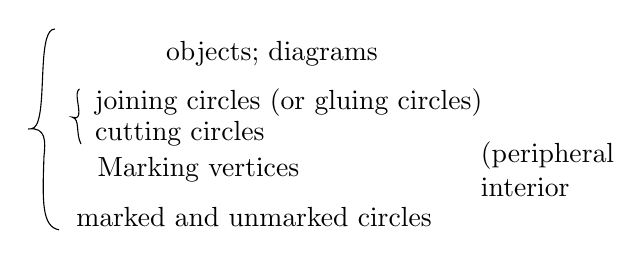
\begin{tikzpicture}[x=1cm,y=1cm,every node/.style={anchor=west,inner sep=0pt,outer sep=0pt}]
\node at (1.65,0) {objects; diagrams};
\node at (0.75,-0.62) {joining circles (or gluing circles)};
\node at (0.75,-1.02) {cutting circles};
\node at (0.78,-1.47) {\uline{Marking} vertices};
\node[align=left] at (5.65,-1.47) {(peripheral\\interior};
\node at (0.51,-2.08) {marked and unmarked circles};
\draw (0.24,0.31) .. controls (0.03,0.32) and (0.12,-0.53) .. (0.03,-0.84)
  .. controls (0.00,-0.95) and (-0.04,-0.96) .. (-0.10,-0.96)
  .. controls (0.13,-0.93) and (0.12,-1.12) .. (0.10,-1.31)
  .. controls (0.08,-1.87) and (0.07,-2.20) .. (0.29,-2.24);
\draw (0.55,-0.45) .. controls (0.48,-0.50) and (0.56,-0.69) .. (0.54,-0.78)
  .. controls (0.53,-0.82) and (0.49,-0.83) .. (0.46,-0.81)
  .. controls (0.56,-0.83) and (0.50,-1.02) .. (0.57,-1.15);
\end{tikzpicture}}

\begin{tabular}{@{}l@{}}
[\deleted{\unsure{of}} ``anabelian''\\
\hspace{1.4em}or ``stability'' condition]
\end{tabular}

\diagram{\begin{tikzcd}[ampersand replacement=\&,column sep=small,row sep=small]
\&\makebox[0pt][r]{\(\deleted{\unsure{SD}}\)\,}\mathcal T\arrow[dl,dash]\arrow[dr,dash]\arrow[rrrr]\&\&\&\&\unsure{t|\mathbb L}\arrow[dl,dash]\arrow[dr,dash]\&\\
S\mathcal T\arrow[dr,dash]\arrow[rr,dash]\&\&D\mathcal T\arrow[dl,dash]\arrow[rr,bend left=15]\arrow[rrrr,bend right=20]\&\&s\unsure{t|\mathbb L}\arrow[dr,dash]\&\&d\unsure{t|\mathbb L}\arrow[dl,dash]\\
\&SD\mathcal T\arrow[rrrr]\&\&\&\&sd\unsure{t|\mathbb L}\&\\
\&\&\&\&\&\text{\makebox[0pt]{combinatorial types}}\&
\end{tikzcd}}

Catalogue of operations $+$ structures

\figure{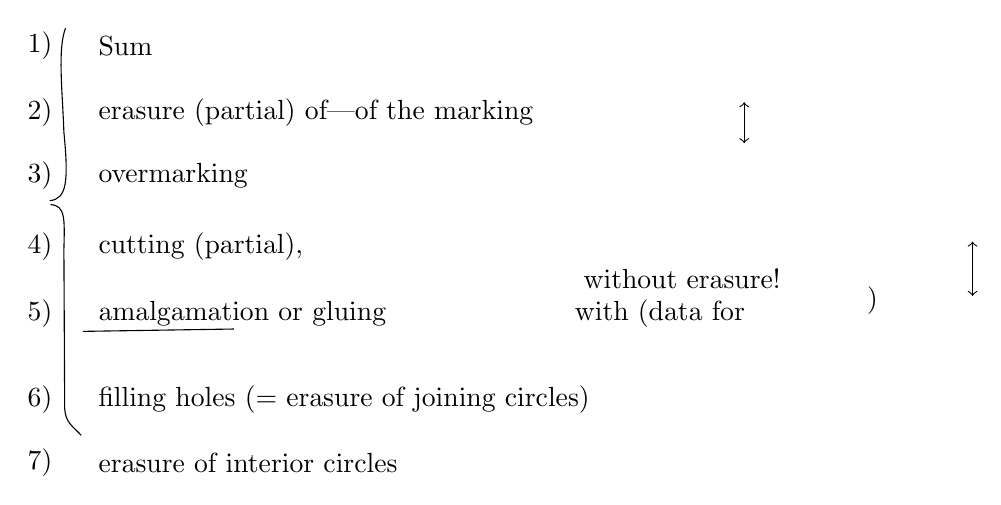
\begin{tikzpicture}[x=1cm,y=1cm,every node/.style={anchor=west,inner sep=0pt,outer sep=0pt}]
\node at (0,0) {1)};
\node at (0.90,0) {Sum};
\node at (0,-0.85) {2)};
\node at (0.90,-0.85) {erasure (partial) \unsure{of|of the} marking};
\node at (0,-1.65) {3)};
\node at (0.90,-1.65) {overmarking};
\draw (0.48,0.22) .. controls (0.38,-0.05) and (0.44,-0.55) .. (0.46,-1.10)
  .. controls (0.52,-1.72) and (0.50,-1.95) .. (0.28,-1.97);
\draw[<->] (9.10,-0.72) -- (9.10,-1.24);
\node at (0,-2.55) {4)};
\node at (0.90,-2.55) {cutting (partial)\unsure{,}};
\node at (0,-3.40) {5)};
\node at (0.90,-3.40) {amalgamation or gluing};
\draw (0.70,-3.63) -- (2.62,-3.60);
\node at (6.95,-3.40) {\deleted{\unsure{with (data for}}};
\node at (7.06,-2.96) {\inserted{without erasure!}};
\node at (10.66,-3.24) {)};
\draw[<->] (12.00,-2.49) -- (12.00,-3.18);
\node at (0,-4.50) {6)};
\node at (0.90,-4.50) {filling holes (= erasure of joining circles)};
\draw (0.29,-2.02) .. controls (0.48,-2.03) and (0.47,-2.20) .. (0.46,-2.59)
  -- (0.47,-4.61) .. controls (0.48,-4.79) and (0.57,-4.83) .. (0.68,-4.95);
\node at (0,-5.30) {7)};
\node at (0.90,-5.30) {erasure of interior circles};
\end{tikzpicture}}

``twist'' functors and isomorphisms
\margin{41}
